\documentclass[11pt]{standalone}

\usepackage{ifthen}
\usepackage{tikz} 
\usetikzlibrary{shapes.misc}
\usetikzlibrary{arrows,arrows.meta}
\usetikzlibrary{calc,intersections, patterns, math}

\definecolor{pfeil}{RGB}{168,167,167}
\definecolor{petrol}{RGB}{0, 118, 136}
\definecolor{darkgoldenrod}{RGB}{184, 134, 11}
\colorlet{petrol-lighter}{petrol!40}
\colorlet{darkgoldenrod-lighter}{darkgoldenrod!40}

\begin{document}

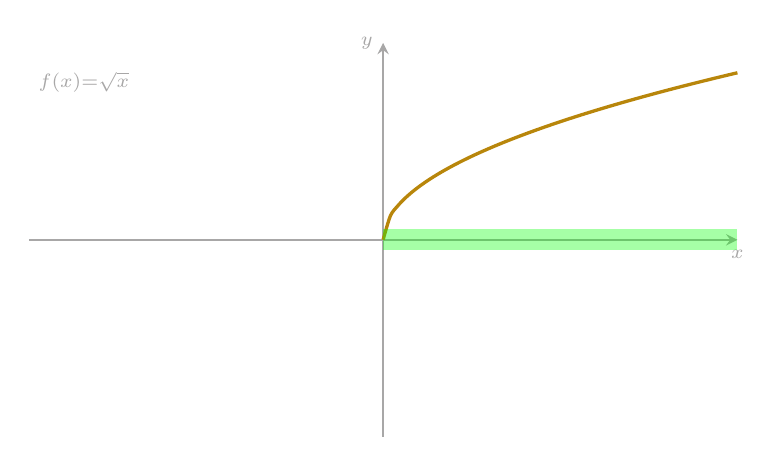
\begin{tikzpicture}[pfeil]

    % \draw[thick, fill=petrol!20, draw=petrol-lighter, rounded corners=2ex, opacity=0.5] (0,0) rectangle ++ (1.5,3.5);
    % \draw[thick, fill=darkgoldenrod!20, draw=darkgoldenrod-lighter, rounded corners=2ex, opacity=0.5] (5,0) rectangle ++ (1.5,3.5);

    \draw[thick, -stealth] (-4.5,0) -- (4.5,0) node[below]{$\scriptstyle x$};
	\draw[thick, -stealth] (0,-2.5) -- (0,2.5) node[left]{$\scriptstyle y$};
	
	\draw[very thick,domain=0:4.5, smooth, samples=50, darkgoldenrod] plot(\x,{sqrt(\x)});

    \draw[line width=7.5px, green, opacity=0.35,-] (0,0) -- (4.5,0);

    % \foreach \x in {1,...,5}{
    %     \draw[] (\x ,0) -- ++ (0,-0.075) node[below, yshift=0.75mm] {\tiny \x0} ;
    % }
    % \foreach \x in {5,10,...,30}{
    %     \draw[] (0, \x/10) -- ++ (-0.075,0) node[left, xshift=0.75mm] {\tiny \x0\,000} ;
    % }
    % }
    \node[right] at (-4.5,2) {$\scriptstyle f(x)=\sqrt{x}$};

\end{tikzpicture}

\end{document}
